\subsection{ ''Notch Depth''}

Se llama $notch$  $depht$ a la profundidad del pico del filtro notch. Esta profundidad es la m\'axima atenuaci\'on que presentar\'a la se\~nal de entrada.

\paragraph*{C\'alculo anal\'itico:} Observando la funci\'on transferencia ideal del circuito, que se transcribe a continuaci\'on:

\begin{equation}
H(s) = \frac{2}{1+k^2} \cdot \frac{s^2 + \left( \frac{k}{RC}\right)^2}{s^2 + \frac{1}{RCQ} s + \left(\frac{1}{RC}\right)^2}
\label{vovi_simple2}
\end{equation}

Se puede decir que dado que el Q del cero es $\infty$, el pico del notch deber\'a tener una atenuaci\'on infinita. Esto es para el caso ideal, el cual no se cumple al momento de medir. Para ver anal\'iticamente lo que ocurre con el pico del notch, se evalu\'o $H(s=j2\pi f)$ para obtener la funci\'on transferencia en funci\'on de la frecuencia en Hz. Luego se tom\'o su m\'odulo y se busc\'o su m\'inimo, obteniendo para este una frecuencia de $1,082kHz$. A esta frecuencia deber\'ia estar te\'oricamente el pico del notch.

\paragraph*{Medici\'on:} Para medir la frecuencia y la atenuaci\'on del pico del notch, primero se intent\'o hacerlo con el bodeador. Al ir achicando el rango de frecuencias en la zona del pico y al exigirle al programa la obtenci\'on de m\'as puntos de medici\'on, se not\'o que la atenuaci\'on del pico iba variando, haciendose cada vez mayor. La atenuaci\'on m\'axima que se logr\'o obtener de esta forma fue de $\approx 30dB$. Este resultado se muestra en el gr\'afico \ref{pico}. En este gr\'afico se compara lo medido con lo te\'orico y con simulaci\'on Montecarlo, pero tambi\'en se contrasta con la simulaci\'on del valor exacto (ideal y deseado) de los componentes elegidos y teniendo en cuenta las puntas. Al estar analizando una zona de detalle, se compar\'o con la simulaci\'on reci\'en aclarada y no solo con el Montecarlo ya que el mismo presenta curvas muy exparsidas y pod\'ia ser relevante observar a qu\'e ser\'a mejor aproximarse y poder entender qu\'e tan lejos o cerca se logr\'o llegar de la frecuencia y de la atenuaci\'on del pico del notch.

\begin{figure}[H] %!ht
	\centering
	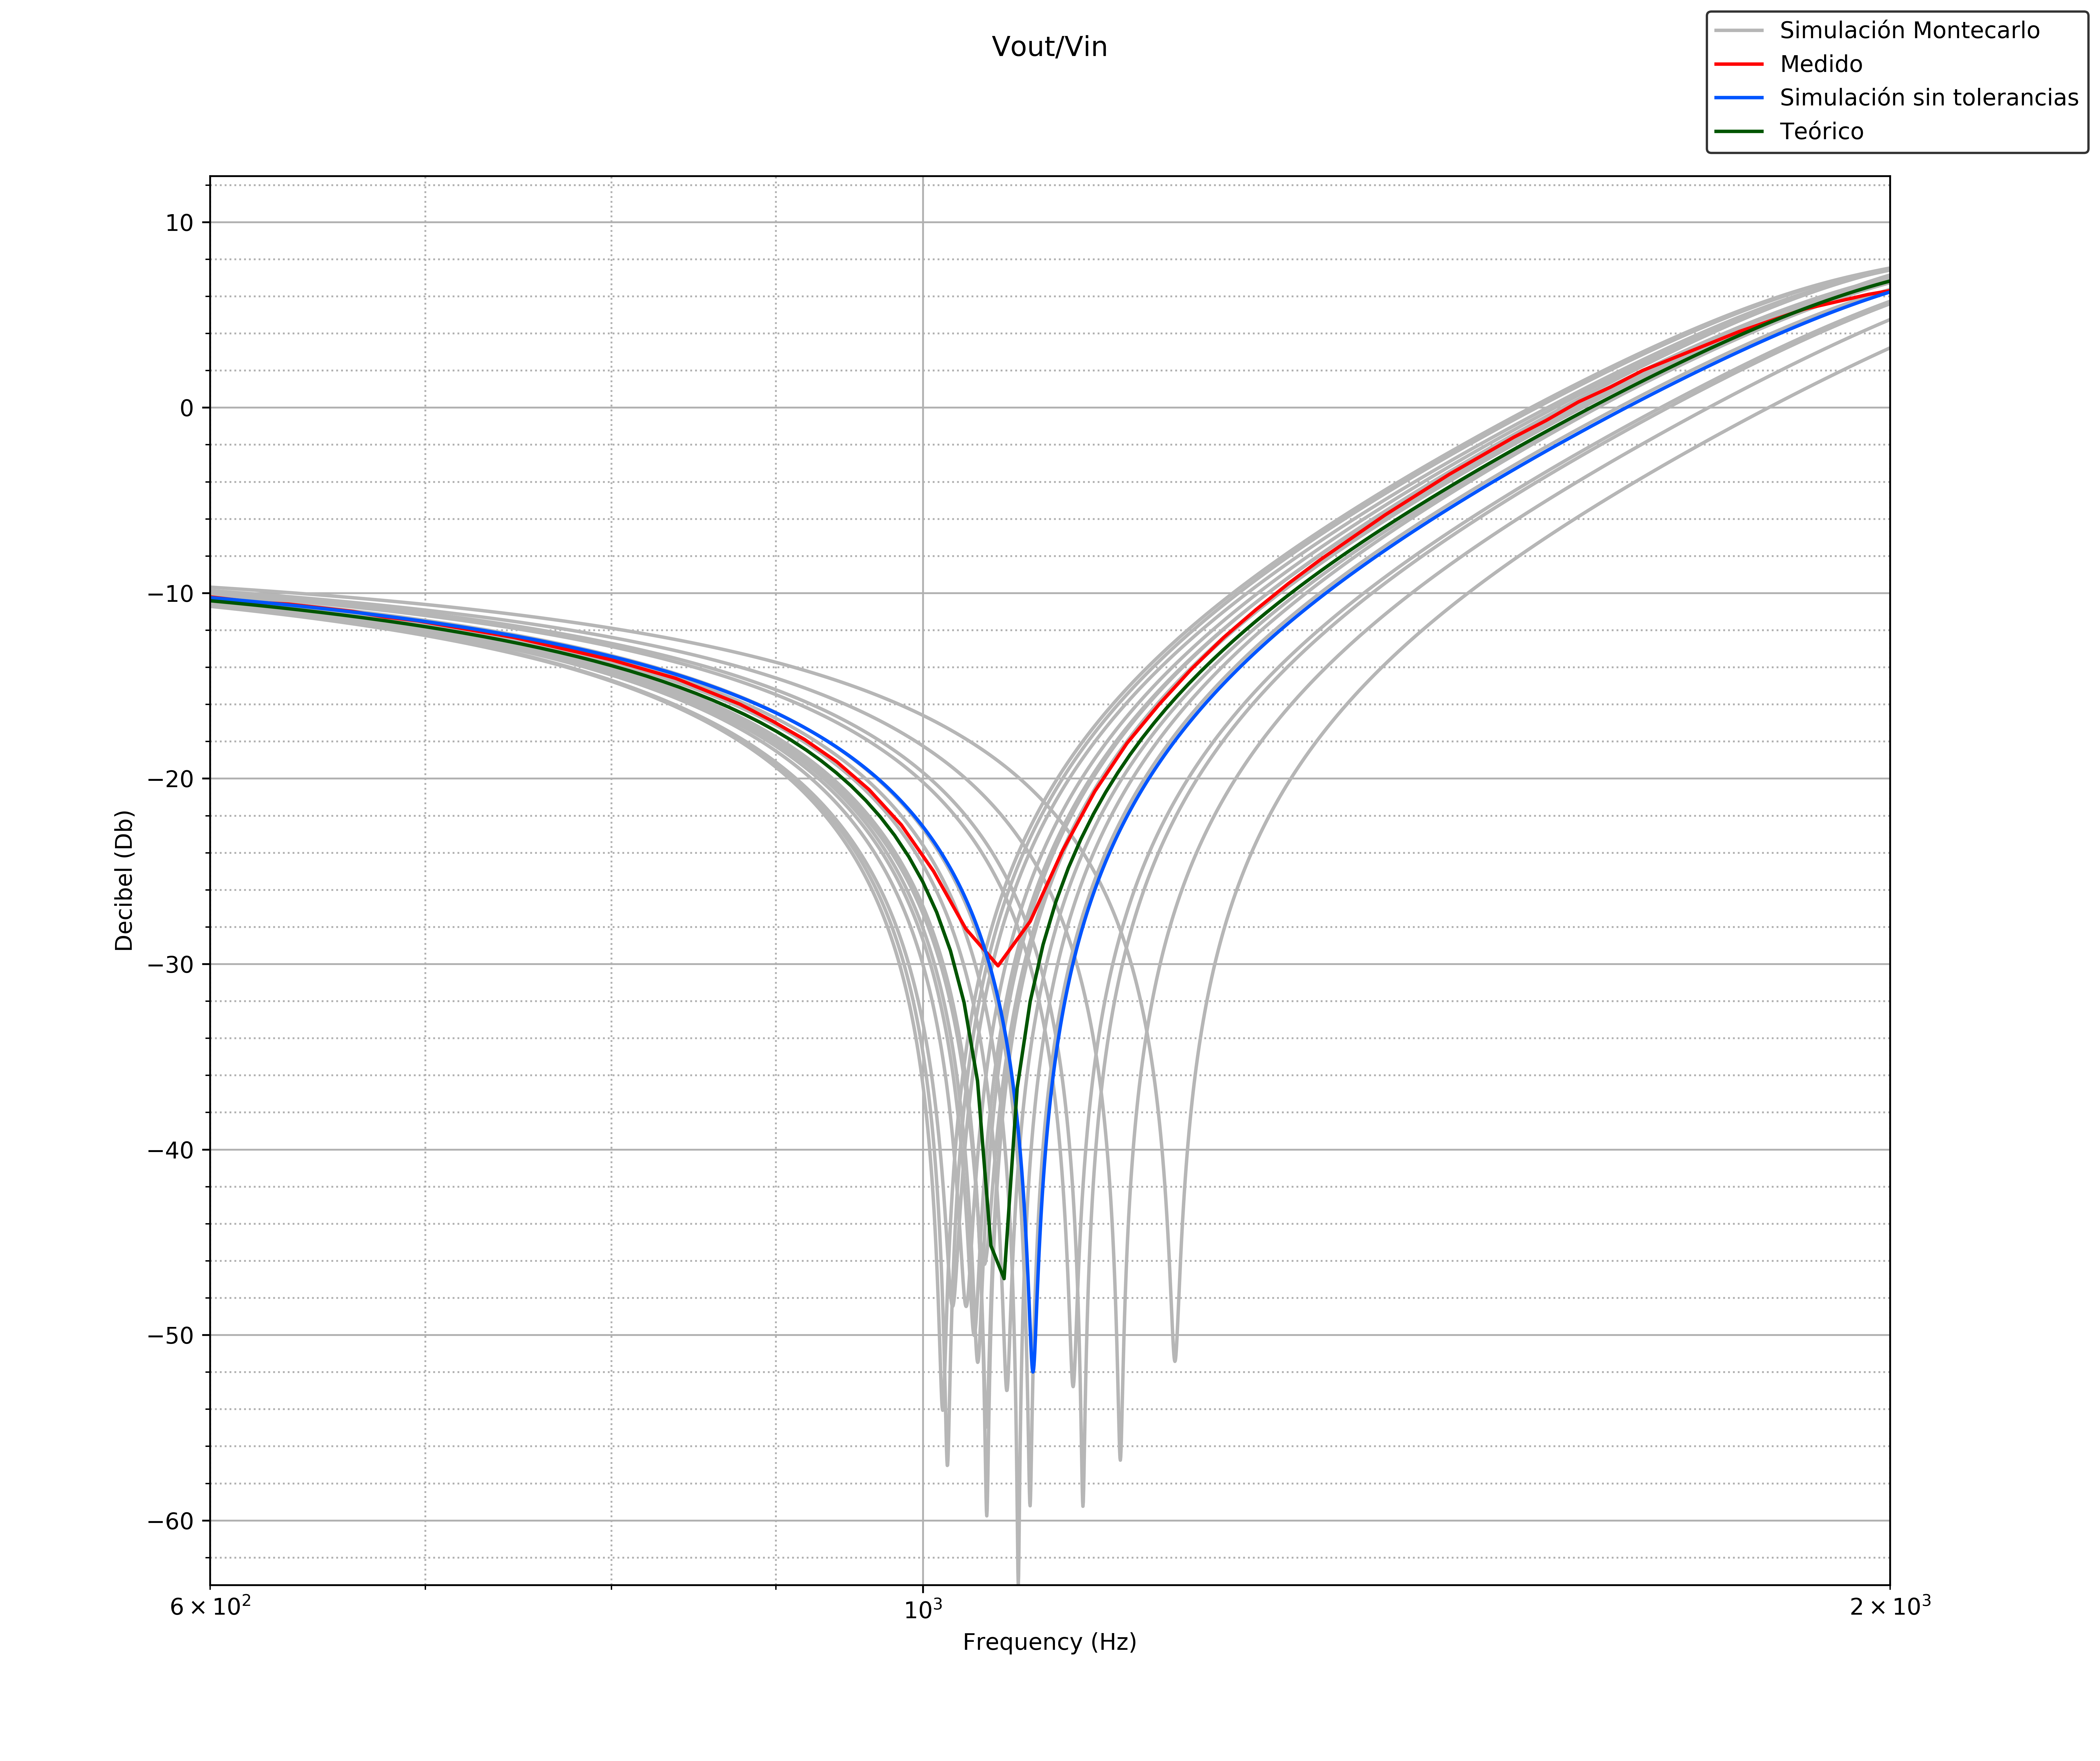
\includegraphics[width=10cm,height=10cm,keepaspectratio]{../EJ1/00GRAFICOS/pico.png}
	\caption{Detalle del pico del notch.}
	\label{pico}
\end{figure}

Al percatarse de que pod\'ian no ser suficientes los puntos tomados en la zona del pico, luego, empleando el osciloscopio manualmente, se busc\'o la frecuencia para la cual la salida es m\'inima, obteniendo $1,097kHz$. Para dicho punto se obtuvo una atenuaci\'on de $\approx35dB$, la cual es menor que la predicha con los c\'alculos te\'oricos al no tratarse de un filtro notch ideal, pero con una atenuaci\'on de $5dB$ m\'as que la previamente obtenida con el bodeador. Por lo tanto, se verific\'o que en el proceso de medici\'on de la funci\'on transferencia este pico tambi\'en se lo vio con menor atenuaci\'on debido al m\'etodo de medici\'on.

